\begin{figure}[!t]
\centering
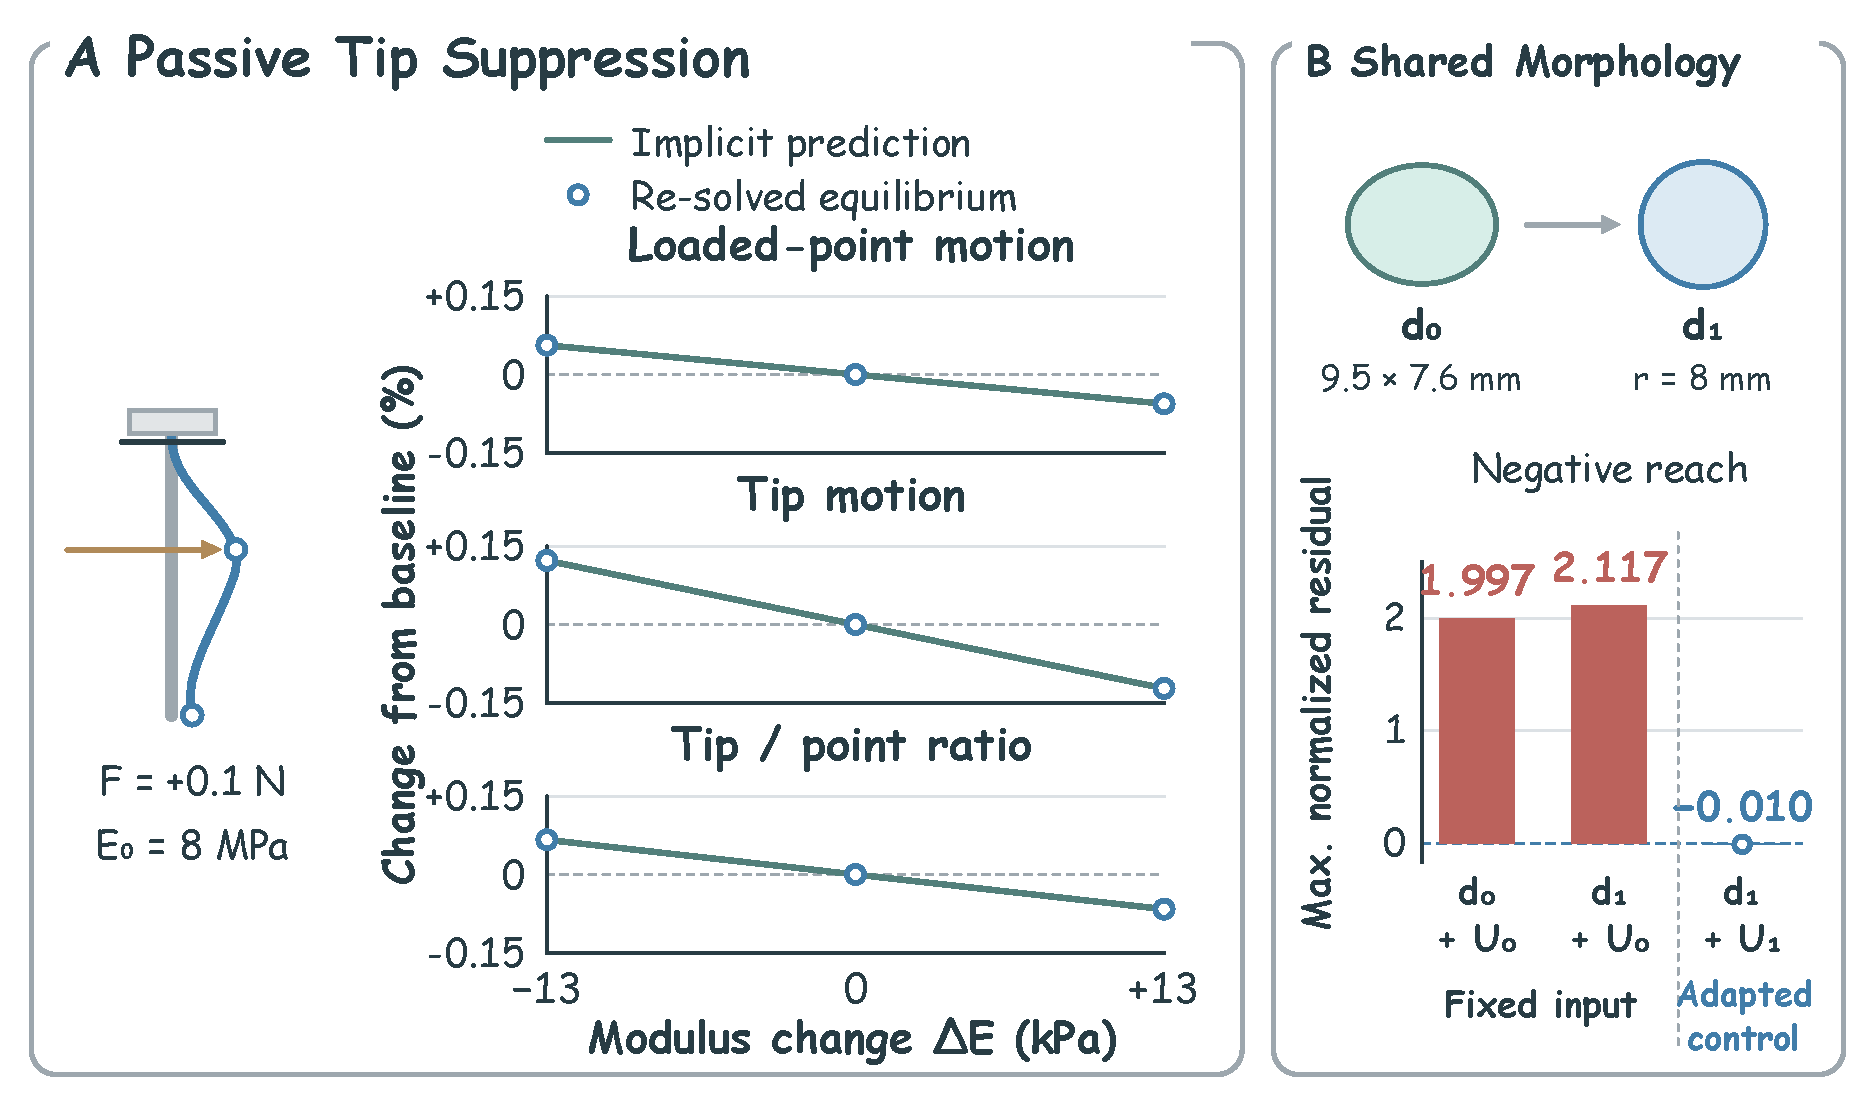
\includegraphics[width=\columnwidth]{figures/fig04_mathematical_research.pdf}
\caption{Task-conditioned mathematical evidence for structural and control refinement. (A) For a representative proximal positive-load condition, implicit equilibrium predictions and re-solved equilibria show the effects of Young's-modulus perturbations on loaded-point motion, projected tip motion, and their ratio. Aggregate agreement across six signed-load branches and three observables is reported in the text. (B) Negative-reach comparison among the original morphology with its original input ($d_0,U_0$), the modified morphology under the same input ($d_1,U_0$), and the modified morphology after control re-optimization ($d_1,U_1$). Bars show the maximum signed normalized task residual; nonpositive values satisfy the condition.}
\label{fig:mathematical-research}
\end{figure}
